\entry{Semana del 14/04/2025}

Ya estaba impreso el prototipo inicial de la carcasa del sensor. Más abajo se muestran un par de fotos de la impresión. 

\begin{figure}[!ht]
	\centering
	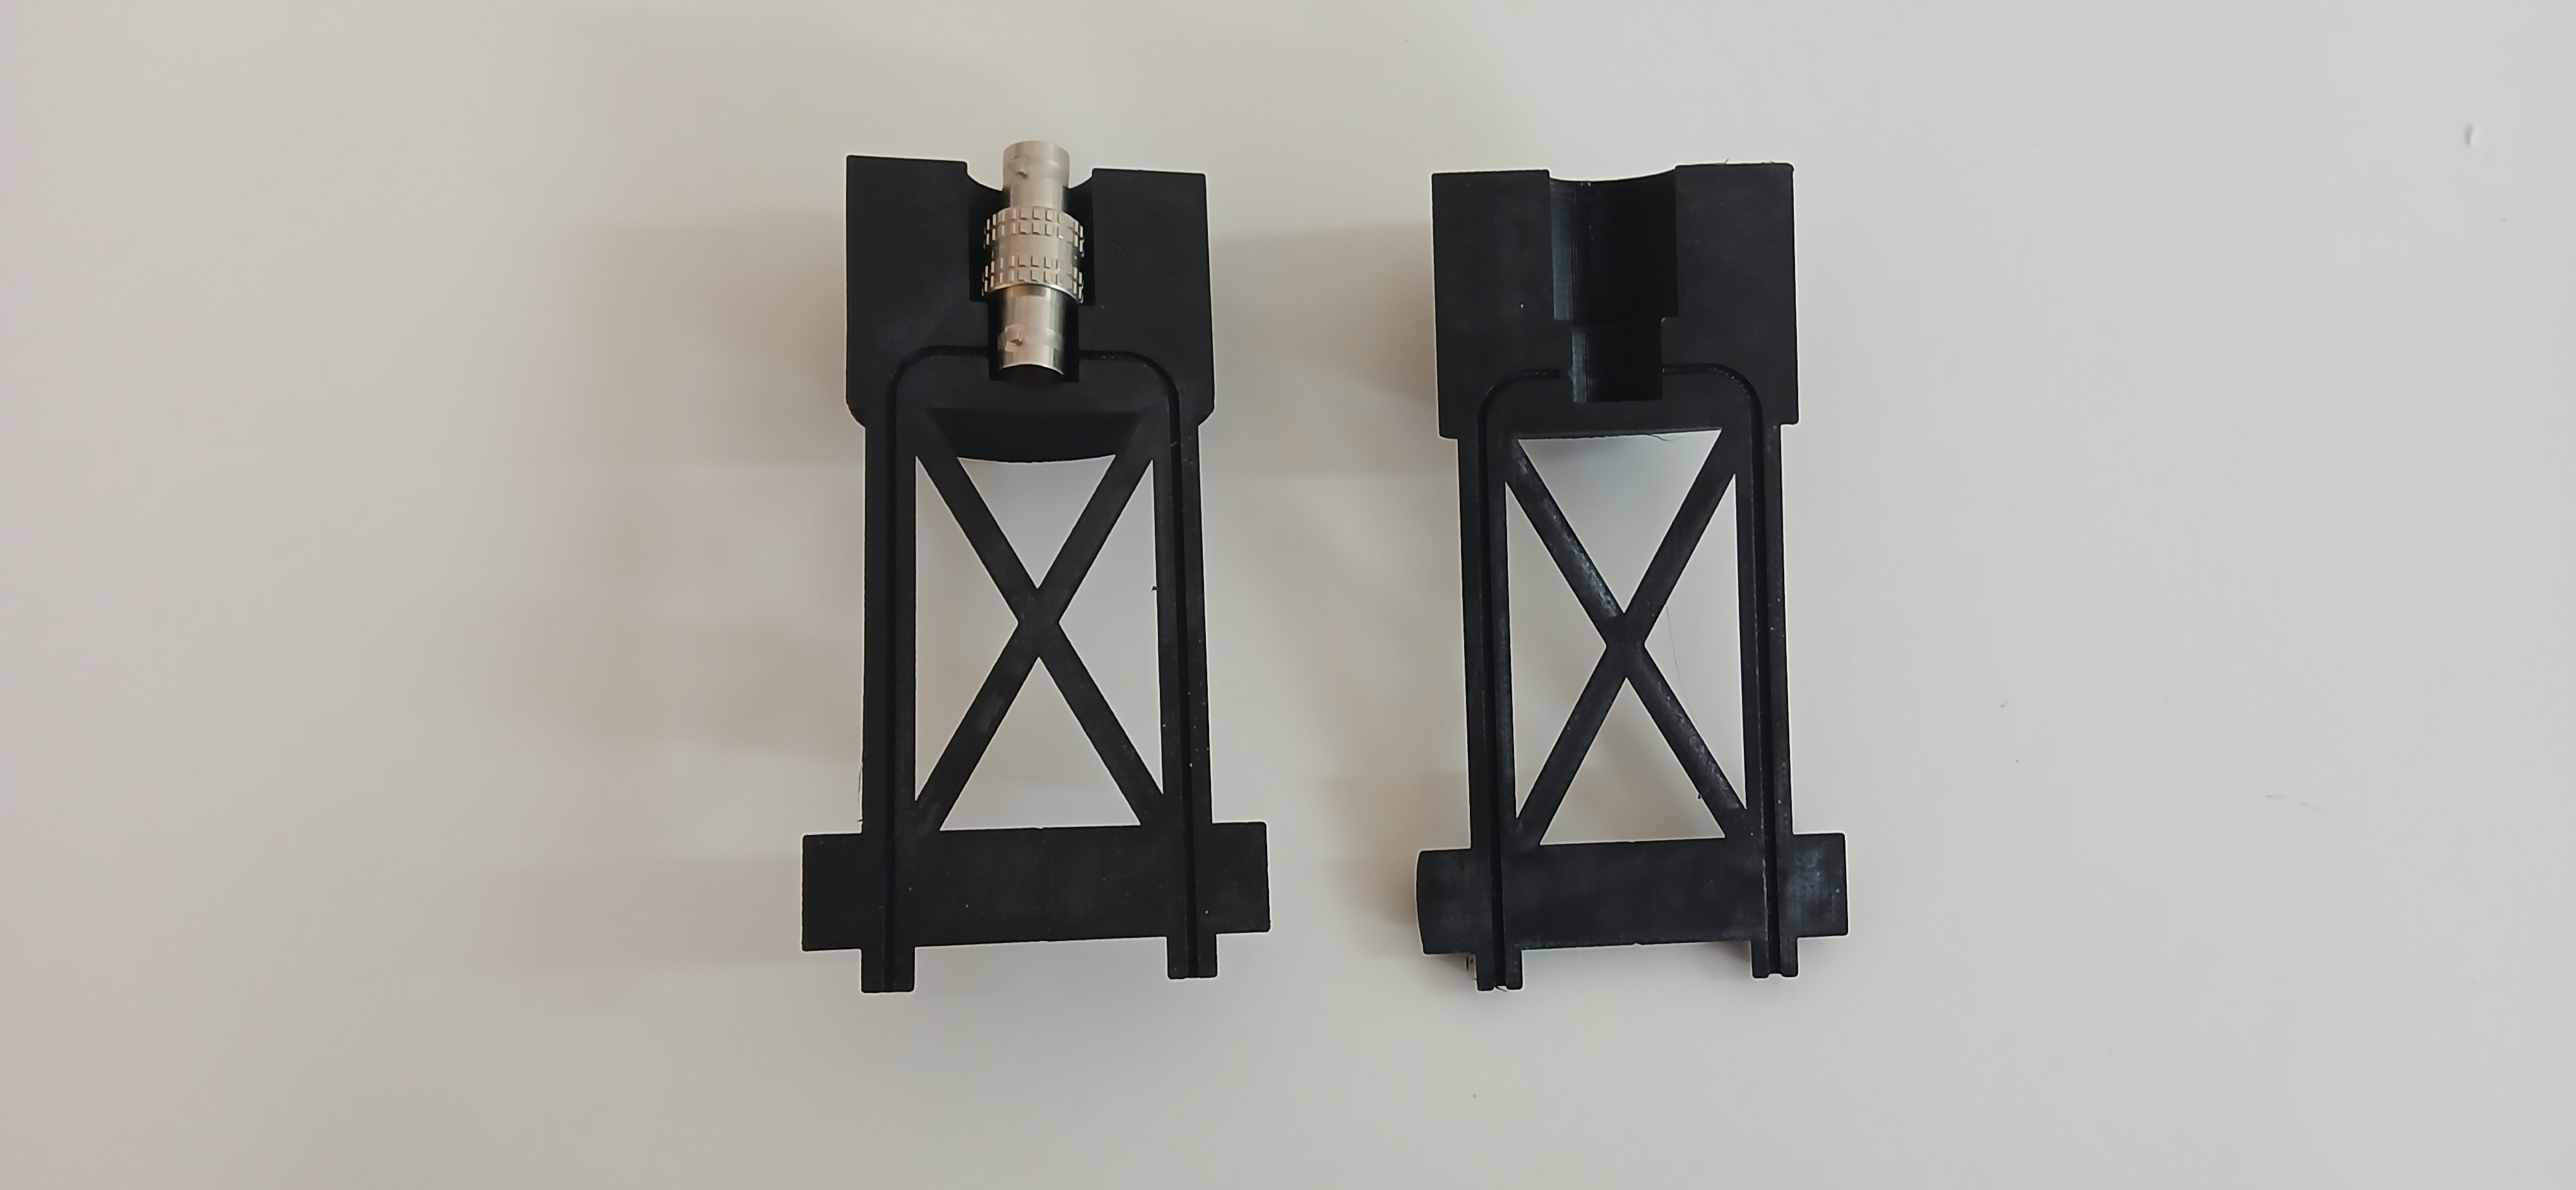
\includegraphics[width=0.97\linewidth]{Figures/14_04_2025/Pieza_impresa}
	\caption{Pieza impresa en 3D.}
	\label{fig:piezaimpresa}
\end{figure}


Un par de consideraciones:  
\begin{itemize}
	\item El agujero para el cable de cobre se cerró, quedó por debajo de la resolución de la impresión.
	\item El agujero para el cable de acero también se achicó igualmente. Quedó de aproximadamente 1.4 mm de diámetro, entrando un cable tipo jumper de la protoboard.
	\item La cabeza de BNC entra perfecto, con un poco de juego, pero entra con las dimensiones deseadas y hace tope donde debería.
	\item Las dos piezas encajan bien entre sí, efectivamente tienen la simetría de reflexión buscada.
	\item El tiempo de impresión (aunque fue en conjunto con otras piezas) fue de 12 hs aproximadamente. Si queremos hacer una cantidad importante en el futuro se puede hacer más hueco para que tarde menos. 
	\item Para cerrarlos se puede pensar en encastre, que se podría romper al intentar volverlos a separar, o tornillos de plástico con tuerca, dos arriba y uno o dos abajo por ejemplo.
\end{itemize}